% Copyright 2016 - 2023 Bas van Meerten and Wouter Franssen and Julien TREBOSC
%
%This file is part of ssNake.
%
%ssNake is free software: you can redistribute it and/or modify
%it under the terms of the GNU General Public License as published by
%the Free Software Foundation, either version 3 of the License, or
%(at your option) any later version.
%
%ssNake is distributed in the hope that it will be useful,
%but WITHOUT ANY WARRANTY; without even the implied warranty of
%MERCHANTABILITY or FITNESS FOR A PARTICULAR PURPOSE.  See the
%GNU General Public License for more details.
%
%You should have received a copy of the GNU General Public License
%along with ssNake. If not, see <http://www.gnu.org/licenses/>.

\documentclass[11pt,a4paper]{article}
% Copyright 2016 - 2017 Bas van Meerten and Wouter Franssen
%
%This file is part of ssNake.
%
%ssNake is free software: you can redistribute it and/or modify
%it under the terms of the GNU General Public License as published by
%the Free Software Foundation, either version 3 of the License, or
%(at your option) any later version.
%
%ssNake is distributed in the hope that it will be useful,
%but WITHOUT ANY WARRANTY; without even the implied warranty of
%MERCHANTABILITY or FITNESS FOR A PARTICULAR PURPOSE.  See the
%GNU General Public License for more details.
%
%You should have received a copy of the GNU General Public License
%along with ssNake. If not, see <http://www.gnu.org/licenses/>.

\usepackage[british]{babel}
\usepackage{graphicx,booktabs,listings,amsmath,pgfplots,pgfplotstable}
\usepackage[small,bf,nooneline]{caption}
\usepackage{subcaption}
\usepackage[sort&compress,numbers]{natbib}
\usepackage{tikz}
\usepackage{mathtools}
\usepackage[nottoc]{tocbibind}%adds bibliography to table of contents.
\graphicspath{{./images/}}
%\setlength{\textwidth}{453pt} %597 pt is the a4 paperwidth. Minus 2 in margin. 72 pt = 1 in
%\setlength{\hoffset}{-\oddsidemargin}
%\setlength{\voffset}{-30pt} %
%\setlength{\textheight}{651 pt} %a4 height 845 pt minus 2* total headheight. In this case 2*88pt
%% examine margines via the layout package. Use command \layout{} in document to draw a picture.
%\setlength{\parindent}{0.5 cm}
%\setlength{\parskip}{0 cm}
\usepackage[left=82pt,right=82pt,top=95pt,bottom=95pt,footnotesep=0.5cm]{geometry}
%\setlength{\headheight}{14pt}

%define colours--------------------
%dark
\usepackage{xcolor}
\definecolor{MyGrayD}{RGB}{1,1,1}
\definecolor{MyRedD}{RGB}{237,45,46}
\definecolor{MyGreenD}{RGB}{0,140,71}
\definecolor{MyBlueD}{RGB}{24,89,169}
\definecolor{MyOrangeD}{RGB}{243,125,34}
\definecolor{MyPurpleD}{RGB}{102,44,145}
\definecolor{MyBrownD}{RGB}{161,29,32}
\definecolor{MyPinkD}{RGB}{179,56,147}
%normal
\definecolor{MyGray}{RGB}{114,114,114}
\definecolor{MyRed}{RGB}{241,89,95}
\definecolor{MyGreen}{RGB}{121,195,106}
\definecolor{MyBlue}{RGB}{89,154,211}
\definecolor{MyOrange}{RGB}{249,166,90}
\definecolor{MyPurple}{RGB}{158,102,171}
\definecolor{MyBrown}{RGB}{205,112,88}
\definecolor{MyPink}{RGB}{215,127,179}
%light
\definecolor{MyGrayL}{RGB}{204,204,204}
\definecolor{MyRedL}{RGB}{242,174,172}
\definecolor{MyGreenL}{RGB}{216,228,170}
\definecolor{MyBlueL}{RGB}{184,210,235}
\definecolor{MyOrangeL}{RGB}{242,209,176}
\definecolor{MyPurpleL}{RGB}{212,178,211}
\definecolor{MyBrownL}{RGB}{221,184,169}
\definecolor{MyPinkL}{RGB}{235,191,217}
%----------------------------------

%Figure ref with hyperref
\newcommand{\fref}[1]{\hyperref[#1]{Figure \ref*{#1}}}
\newcommand{\sref}[1]{\hyperref[#1]{Section \ref*{#1}}}
\newcommand{\tref}[1]{\hyperref[#1]{Table \ref*{#1}}}

%Makes a new command for figures with input values: filename, width(times linewidth),
% caption and label.
\newcommand{\onefigure}[4]{
\setlength{\captionwidth}{#2\linewidth}
\begin{figure}
\includegraphics[width=#2\linewidth]{#1}
\centering
\parbox{\linewidth}{\caption{#3}
\label{#4}}
\end{figure}
}

%Makes a new command for tikz figures with input values: tikz commands, 
% caption and label.
\newcommand{\onetikz}[3]{
\settowidth{\captionwidth}{#1}
\ifthenelse{\lengthtest{\captionwidth<0.7\linewidth}}{\setlength{\captionwidth}{0.7\linewidth}}{}

\begin{figure}
\centering
#1
\centering
\parbox{\linewidth}{\caption{#2}
\label{#3}}
\end{figure}
}

%Makes a new command for two figures next to each other with input values: filename1, caption1, label1,filename2, caption2 and label2. Figure width is set to 0.47\linewidth and the space between the figures is filled with \hfill so the sides of the figures align with to edge of the line.
\newcommand{\twofigure}[6]{
\setlength{\captionwidth}{\linewidth}
\begin{figure*}[ht!]
\begin{minipage}[t]{0.47\linewidth}
\includegraphics[width=\linewidth]{#1}
\centering
\caption{#2}
\label{#3}
\end{minipage}
\hfill
\begin{minipage}[t]{0.47\linewidth}
\centering
\includegraphics[width= \linewidth]{#4}
\centering
\caption{#5}
\label{#6}
\end{minipage}
\end{figure*}
}


%Makes a new command for a table with caption witdh equal to the total table width. Input: tabular, caption and label. Example:
%\onetable{
%\begin{tabular}{ccc}
%a&b&c\\
%\hline
%1&1&1\\
%1&1&1\\
%1&1&1\\
%\end{tabular}
%{The caption.}
%{tab:table1}
%}
\newcommand{\onetable}[3]{
\settowidth{\captionwidth}{#1}
\ifthenelse{\lengthtest{\captionwidth<0.7\linewidth}}{\setlength{\captionwidth}{0.7\linewidth}}{}
\begin{table}
\caption{#2}
\vspace{-0.24cm} %Puts caption close to toprule
\label{#3}
\centering
#1
\end{table}
}

%Makes a long table with captionwidth equal to tablewidth. It takes the following arguments:
%1: Column specifier (e.g. cccc)
%2: Caption
%3: Label
%4: First head (i.e. first row of regular table)
%5: Head of consecutive pages
%6: Foot of pagebreak
%7: Lastfoot (e.g. \midrule)
%8: Body of table
\newcommand{\onelongtable}[8]{
\begin{center}
\settowidth{\captionwidth}{
\begin{tabular}{#1}
#4
#8
\end{tabular}} % This ends the captionwidth part. Next comes the real table.

\begin{longtable}{#1}
\caption{#2}\\
\vspace{-0.74cm} %Puts caption close to toprule
\label{#3}\\

#4
\endfirsthead

#5
\endhead

#6
\endfoot

#7
\endlastfoot

#8
\end{longtable}
\end{center}}




%1:pgfplots code
%2:width
%3:caption
%4:label
\newcommand{\pgfplotsfigure}[4]{
\pgfplotsset{width=#2\linewidth}
\setlength{\captionwidth}{#2\linewidth}
\begin{figure}[t]
\centering
#1
\centering
\parbox{\linewidth}{\caption{#3}
\label{#4}}
\end{figure}
}


\usepackage[bitstream-charter]{mathdesign}
\usepackage[T1]{fontenc}
\usepackage[protrusion=true,expansion,tracking=true]{microtype}
\pgfplotsset{compat=1.7,/pgf/number format/1000 sep={}, axis lines*=left,axis line style={gray},every outer x axis line/.append style={-stealth'},every outer y axis line/.append style={-stealth'},tick label style={font=\small},label style={font=\small},legend style={font=\footnotesize}}
\usepackage{colortbl}
\usetikzlibrary{calc}

%Set section font
\usepackage{sectsty}
\allsectionsfont{\color{black!70}\fontfamily{SourceSansPro-LF}\selectfont}
%--------------------


%Set toc fonts
\usepackage{tocloft}
%\renewcommand\cftchapfont{\fontfamily{SourceSansPro-LF}\bfseries}
\renewcommand\cfttoctitlefont{\color{black!70}\Huge\fontfamily{SourceSansPro-LF}\bfseries}
\renewcommand\cftsecfont{\fontfamily{SourceSansPro-LF}\selectfont}
%\renewcommand\cftchappagefont{\fontfamily{SourceSansPro-LF}\bfseries}
\renewcommand\cftsecpagefont{\fontfamily{SourceSansPro-LF}\selectfont}
\renewcommand\cftsubsecfont{\fontfamily{SourceSansPro-LF}\selectfont}
\renewcommand\cftsubsecpagefont{\fontfamily{SourceSansPro-LF}\selectfont}
%--------------------

%Define header/foot
\usepackage{fancyhdr}
\pagestyle{fancy}
\fancyhead[LE,RO]{\fontfamily{SourceSansPro-LF}\selectfont \thepage}
\fancyhead[LO,RE]{\fontfamily{SourceSansPro-LF}\selectfont \leftmark}
\fancyfoot[C]{}
%--------------------

%remove page number from first chapter page
\makeatletter
\let\ps@plain\ps@empty
\makeatother
%----------------------
\usepackage{blindtext, color}
\definecolor{gray75}{gray}{0.75}
\newcommand{\hsp}{\hspace{20pt}}



\usepackage[hidelinks,colorlinks,allcolors=black, pdftitle={T2fitting},pdfauthor={Julien\ Trébosc}]{hyperref}

\interfootnotelinepenalty=10000 %prevents splitting of footnote over multiple pages
\linespread{1.2}

%\usepgfplotslibrary{external}%creates all external tikz images that are included.
%\tikzexternalize[shell escape=-enable-write18]%activate externalization
%\tikzsetexternalprefix{GeneratedFigures/}
%\tikzset{external/force remake} %Enable forced remake

\title{\color{black}\fontfamily{SourceSansPro-LF}\bfseries Fitting a pseudo 2D spectrum to extract T2 in ssNake}
\author{}
\date{\color{black}\fontfamily{SourceSansPro-LF}\bfseries \today}

\begin{document}
%\newgeometry{left=72pt,right=72pt,top=95pt,bottom=95pt,footnotesep=0.5cm}
\microtypesetup{protrusion=true} % enables protrusion

\maketitle

\section{Introduction}
This tutorial will go through processing of 2D dataset, fitting a 1D spectrum using Czjzek model, extracting the amplitude of subsequent 1D
 in the pseudo 2D dataset, then fit the amplitudes vs time with the `Relaxation Curve' model. 
The objective is to see how to extract parameters from a series of fits in order to fit them.

You don't need to have done the CzjzekFitting tutorial before.

\section{Dataset and sample information}

For this tutorial, we will use a $\mathrm{{}^{27}Al}$ spectrum recorded with a hahn echo pulse sequence. 
The data was acquired on a 18.8~T Bruker spectrometer under 20~kHz Magic Angle Spinning.
The pulse sequence is $\mathrm{ P90 - \tau - P180 - \tau - acquisition}$.
The FID is recorded from the top of the echo. \\
It was saved as a pseudo 2D dataset varying the echo delay. The initial echo delay was $\tau=5$ rotor periods (250~µs)
and the delay was incremented by $\tau=5$ rotor periods (250~µs) for subsequent rows. T2 relaxation occurs during $2 \times \tau$.

The sample is mesoporous alumina $\mathrm{Al_2O_3}$ provided by Cláudia Morais. %Sample is aslo $\mathrm{{}^{17}O}$ enriched .
On the 1D spectra you can see 3 sites with typical Czjzek distribution pattern. 4 coordinated aluminum site $\mathrm{Al_{IV}}$ 
at about 65~ppm, five coordinated aluminum site $\mathrm{Al_{V}}$ at about 36~ppm and 6 coordinated aluminum site $\mathrm{Al_{VI}}$
at about 9~ppm.

In such case fitting the 3 sites is mandatory as using integral or peak picking would produce biased value due to overlapping sites.

\section{Processing}
Open the dataset choosing the `ser' file in data/2 folder. Switch to ppm units if not default.
Stay on the 1D plot mode.\\
First use zero filling (Matrix $\rightarrow$ Sizing) and choose 2048 point size. \\
Second, correct for digital filter (Tools $\rightarrow$ Correct Digital Filter). The digital filter part will be shifted to the end of the FID.\\
Do Fourier Transform (ctrl-f) and rephase the spectrum (Tools $\rightarrow$ Phasing $\rightarrow$ Autophase 0th).\\
Correct baseline (Tools $\rightarrow$ Baseline Correction), excluding region 200~ppm $\rightarrow$ -200~ppm. Fit with a polynomial or sine/cosine function of degree 2 or 3. 
Check the `Fit traces separately' button.
Validate with `Ok'.

\section{Fitting the first spectrum with Czjzek model}
This is similar to Czjzek Fitting tutorial. If you are familiar with it you can probably skip this section.

Select the `Fitting $\rightarrow$ Czjzek' fitting model. We will use 3 sites with approximate chemical shift of 75~ppm, 43~ppm and 12~ppm and about 7~ppm of 
chemical shift distribution. In general, the chemical shift lies on the left hand side of second order quadrupolar lineshape. This also applies to Czjzek distribution and is 
only moderated by chemical shift distribution. Remember that gaussian broadening models chemical shift distribution and lorentzian broadening models relaxation!
In such sample relaxation is usually negligeable, we can leave lorentzian broadening to the default 10~Hz value. Fix (check the box) Lorentzian broadening and free 
(uncheck the box) gaussian broadening.

Now we need to pre-calculate a spectrum library to fit the Czjzek distribution. Click on `Library' button. Select the correct spin number (5/2 for $\mathrm{{}^{27}Al}$).
Choose MAS: `infinite MAS' and keep `Satellites' button unchecked as no satellite spinning sideband is visible. Click on `Generate' button to create the libray in memory.

We can now run a simulation by clicking `Sim' button. However, with default $\sigma$ value of 1~MHz, the typical right hand side tail is not visible. 
We need to increase the $\mathrm{Cq}$ distribution ($\sigma$). You can try $\sigma$ = 2, 3, 4 or 5 for site 1 but the lineshape will not change to the expected shape.
This is because the library is not adequate as can be seen by clicking the `show' button. Maximum $\mathrm{Cq}$ calculated for the distribution is 4~MHz by default. 
We need to increase it to a value about $4\times\sigma$ and the average Cq in the distribution is about $\mathrm{C_q} = 2 \sigma$. 
You will need a maximum  $\mathrm{Cq}$ of about 20~MHz.
We can further refine the simulation accounting for real spinning speed as one observe tiny spining sidebands. For that we open the Library window and change to MAS: 
`Finite MAS'. Set spinning speed to 20~kHz. \#sidebands 16 is more than enough as sidebands are very small (this is a parameter for which convergence should be checked!).
`Generate' the library again. Then refine the fit clicking `Fit' again. The fit result can
be see in Fig. \ref{fig:FinalFit_1D}. At that point, I suggest to export the fit `Parameters to file' via the `Import/Export' button.

\begin{figure}[h!]
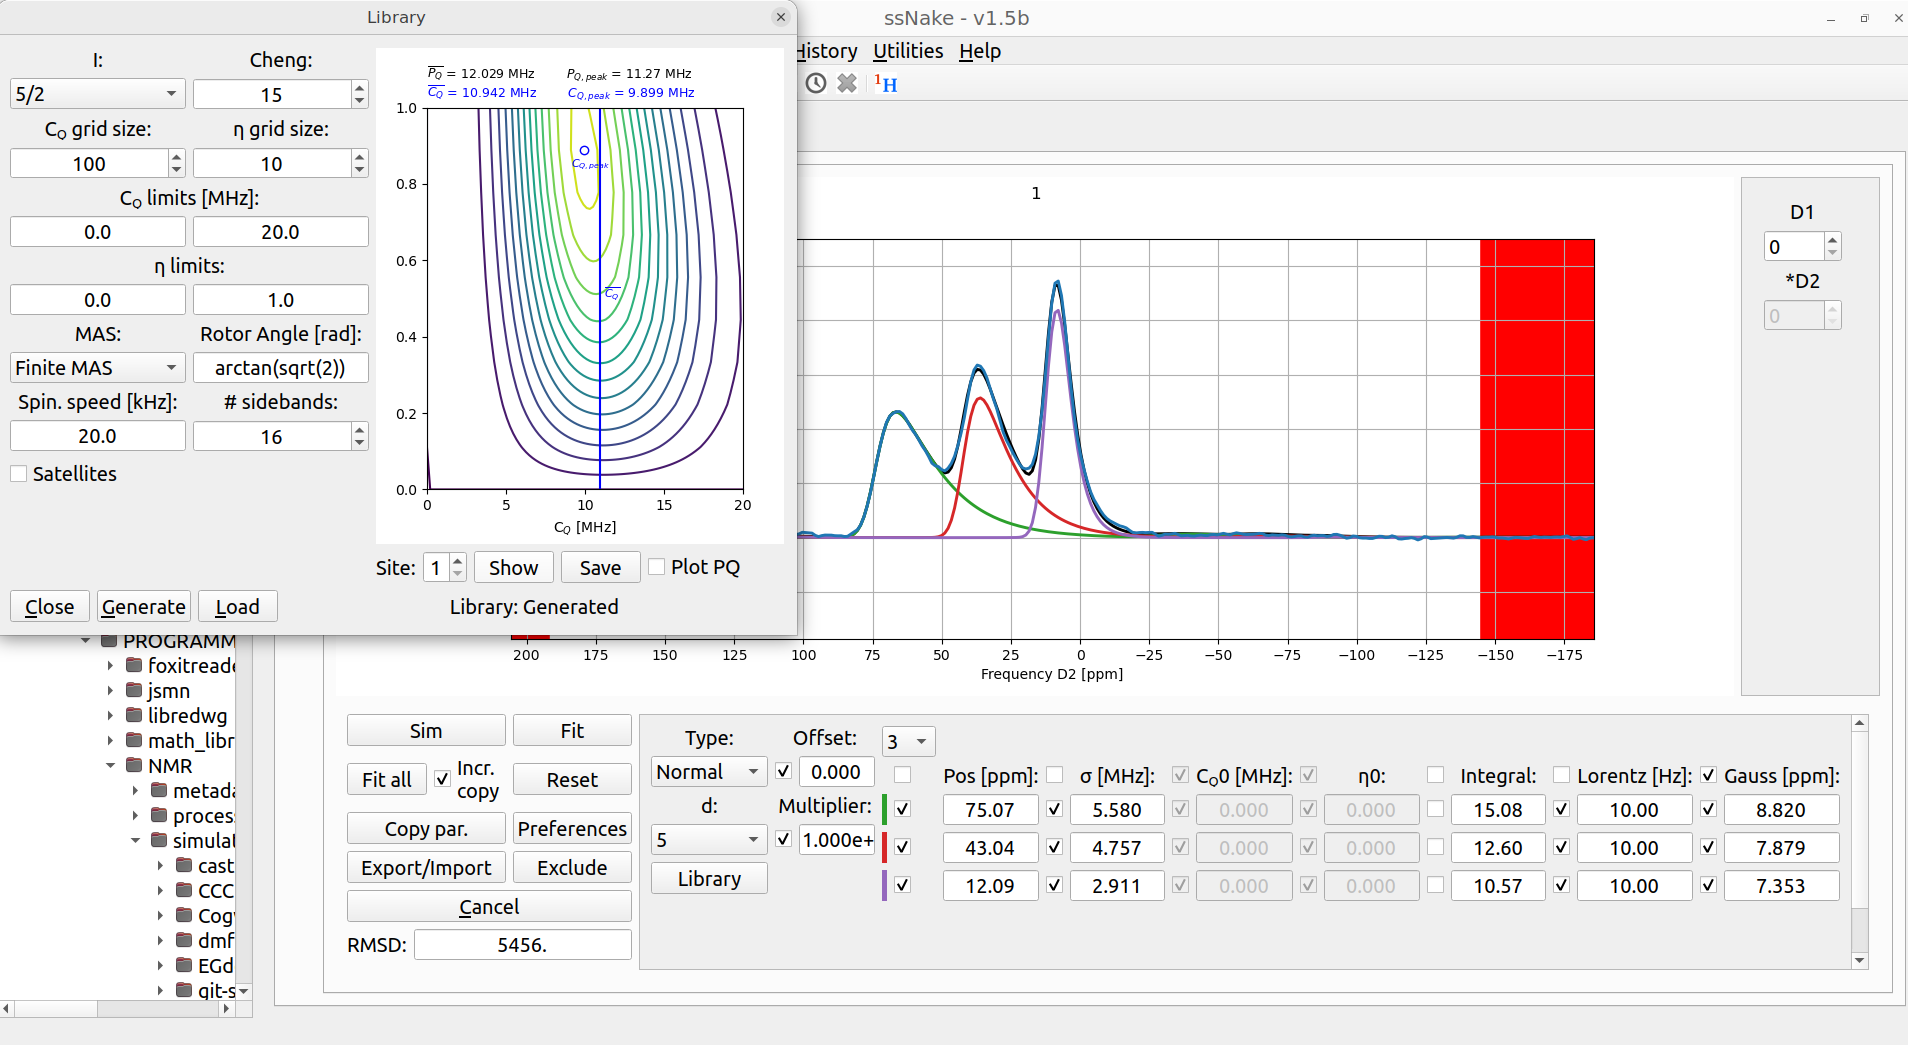
\includegraphics[width=0.8\linewidth]{Figs/FinalFit_1D.png}
\caption{}
\label{fig:FinalFit_1D}
\end{figure}

You will also find good fitting parameters that you can import in `data/2/pdata/1/Al2O3\_JF3\_fit.txt' file to reproduce this figure.

\section{Fitting all spectra for integral}
Now that the first 1D spectrum is properly fitted we will use this fit to get the integral of all three sites in all spectra. 
If you scroll through D1 dimension (spin button on right hand side of the spectrum), you will notice that subsequent rows of the pseudo 2D have initial fitting parameters.\\ 
Come back to row 0 and check all parameter buttons except for the integral parameter. This can be done for all sites for each parameter selecting the parameter name check button. 
(Export again the 1D fit parameters to file...)\\
We now need to copy the first row parameters to other rows: 
Click on `Copy par' button.

You can now click on `Fit all' button to run the fitting procedure for each row. You may need to repeat several times the `Fit all' action if convergence is not reached.
Go through the different rows to verify the different fits.

One problem that can arise is that for large numbered rows, the starting point of the fit is far from convergence.
Generally, the spectra are evolving smoothly from one row to the next one. Therefore a better approach is to copy the parameters from previous row.
In a T2 measurement, the amplitude of the spectra is monotically decreasing. So starting from row 0 we will check the `Incr. copy' check button. 
When not checked `Fit all' fits all rows without performing parameter copy. When `Incr copy' is checked a fit/copy procedure is done: fit row 0 
then copy the fitted parameters to next row, fit row 1, copy fitted parameters to row 2 and so on...\\
If one needs to refine further the fit for each row, subsequent call to `Fit all' should be done with `Incr. copy' option unchecked.

Once the fit for all rows is satisfactory one can export the amplitude parameter to new workspace. From  `Import/Export' window select `Parameters to workspace'.
Then check `Export all slices' and `Integrals' boxes before clicking `Ok'. You can give an explicit name to the new workspace like 'T2s'.

We now have 3D pseudo dataset. D3 dimension contains echo time, D2 dimension holds the different sites (3 rows [0..2] for 3 sites), D1 dimension holds the 
different parameters that were exported to workspace. In our case only integrals were exported so there is only one row for this dimension.

We need to check that the echo time scale is correct. In our dataset the initial echo delay between 90° pulse and 180° pulse was 5 rotor period 
(i.e. 250~µs under 20~kHz MAS). The total echo delay was therefore at 10 rotor periods (500~µs) and the increment the same.
We need to redefine the x axis scale. An increment of 500~µs second corresponds to a spectral window of 2~kHz. So you can set 2~kHz in the Sweepwidth entry.
The starting value remains 0 but this won't affect the T2, but only the initial amplitude. If you need to get the correct amplitude also, then you need to 
use the `Plot $\rightarrow$ User X-axis' menu to define the time x-axis.
Select the linear input and set the start and stop time values in seconds:\\
start value 500e-6, stop value 500e-4 (we have 100 points) and click `Ok'.

\section{Fitting T2 decay curves }
\subsection{Exporting extracted parameters}
Now, data is ready to be used for T2 fitting. One could want to export the data in text mode to process them further in third party software.
This can only be done on 1D or 2D data. But our data is currently 3D. So we need to extract a 2D slice. This can be done using the menu 
`Workspace  $\rightarrow$ Slice to workspace'. The plotted data must be in stack plot or 2D contour mode, not in 1D slice 
otherwise only a 1D spectrum would be sliced to a new workspace. Now we can export the new workspace with 
`File $\rightarrow$ Export $\rightarrow$ ASCII (1D/2D) or CSV(1D/2D)' menu. The CSV (Comma Separated Values) data will appear in columns :\\
Time, Site1\_real, Site1\_imag, Site2\_real, site2\_imag, site3\_real, site3\_imag.

\subsection{T2 fitting}
Let's fit the T2 decay. Select menu `Fitting $\rightarrow$ Relaxation curves'.
We need to fit data with an exponential decay function. We will fix the `Constant' to 0  and the `Coefficient' to 1. Check the box beside them not to fit these parameters.
One can fit the first site T2. Finally, click `Copy par.' then `Fit all' several times to reach reasonable convergence.
As seen in figure \ref{fig:FinalFit_relax}, you should find T2 value of 7.8~ms, 6.4~ms and 4~ms for sites 1 ($\mathrm{Al_{IV}}$), 2 ($\mathrm{Al_{V}}$) and 3 
($\mathrm{Al_{VI}}$) respectively.

\begin{figure}[h!]
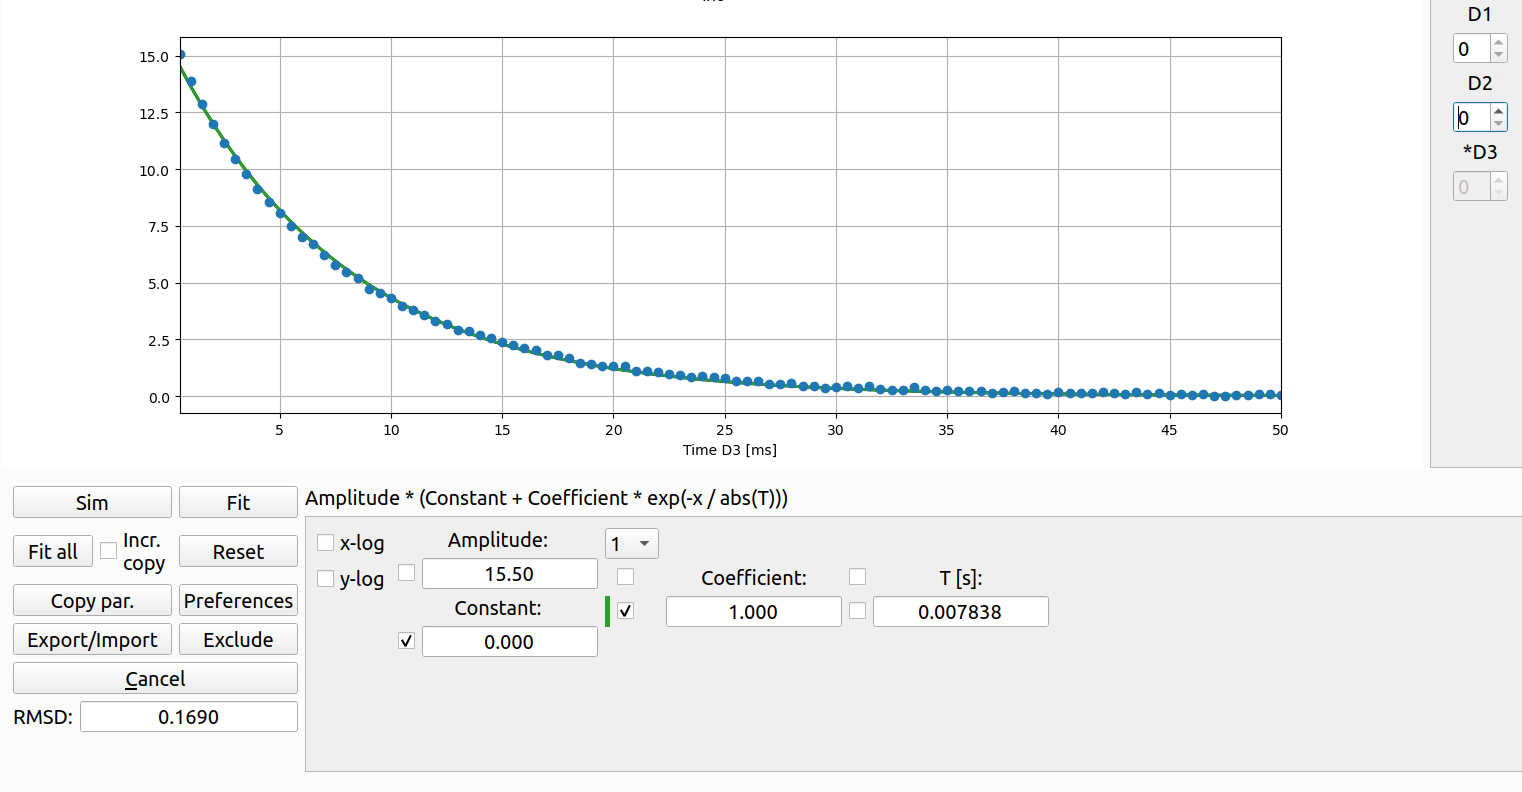
\includegraphics[width=0.8\linewidth]{Figs/FinalFit_relax.png}
\caption{}
\label{fig:FinalFit_relax}
\end{figure}

As $\mathrm{{}^{27}Al}$ is quadrupolar spin, there might be more than one decay component for T2. Also, the peaks seem to shift slightly with echo delay
indicating that there might be more components or that low $C_q$ in the distribution relax faster.
Further exercice: try to fit relaxation with 2 components releasing the Coefficient parameters and fixing the Amplitude.
%%%
%\begin{center}
%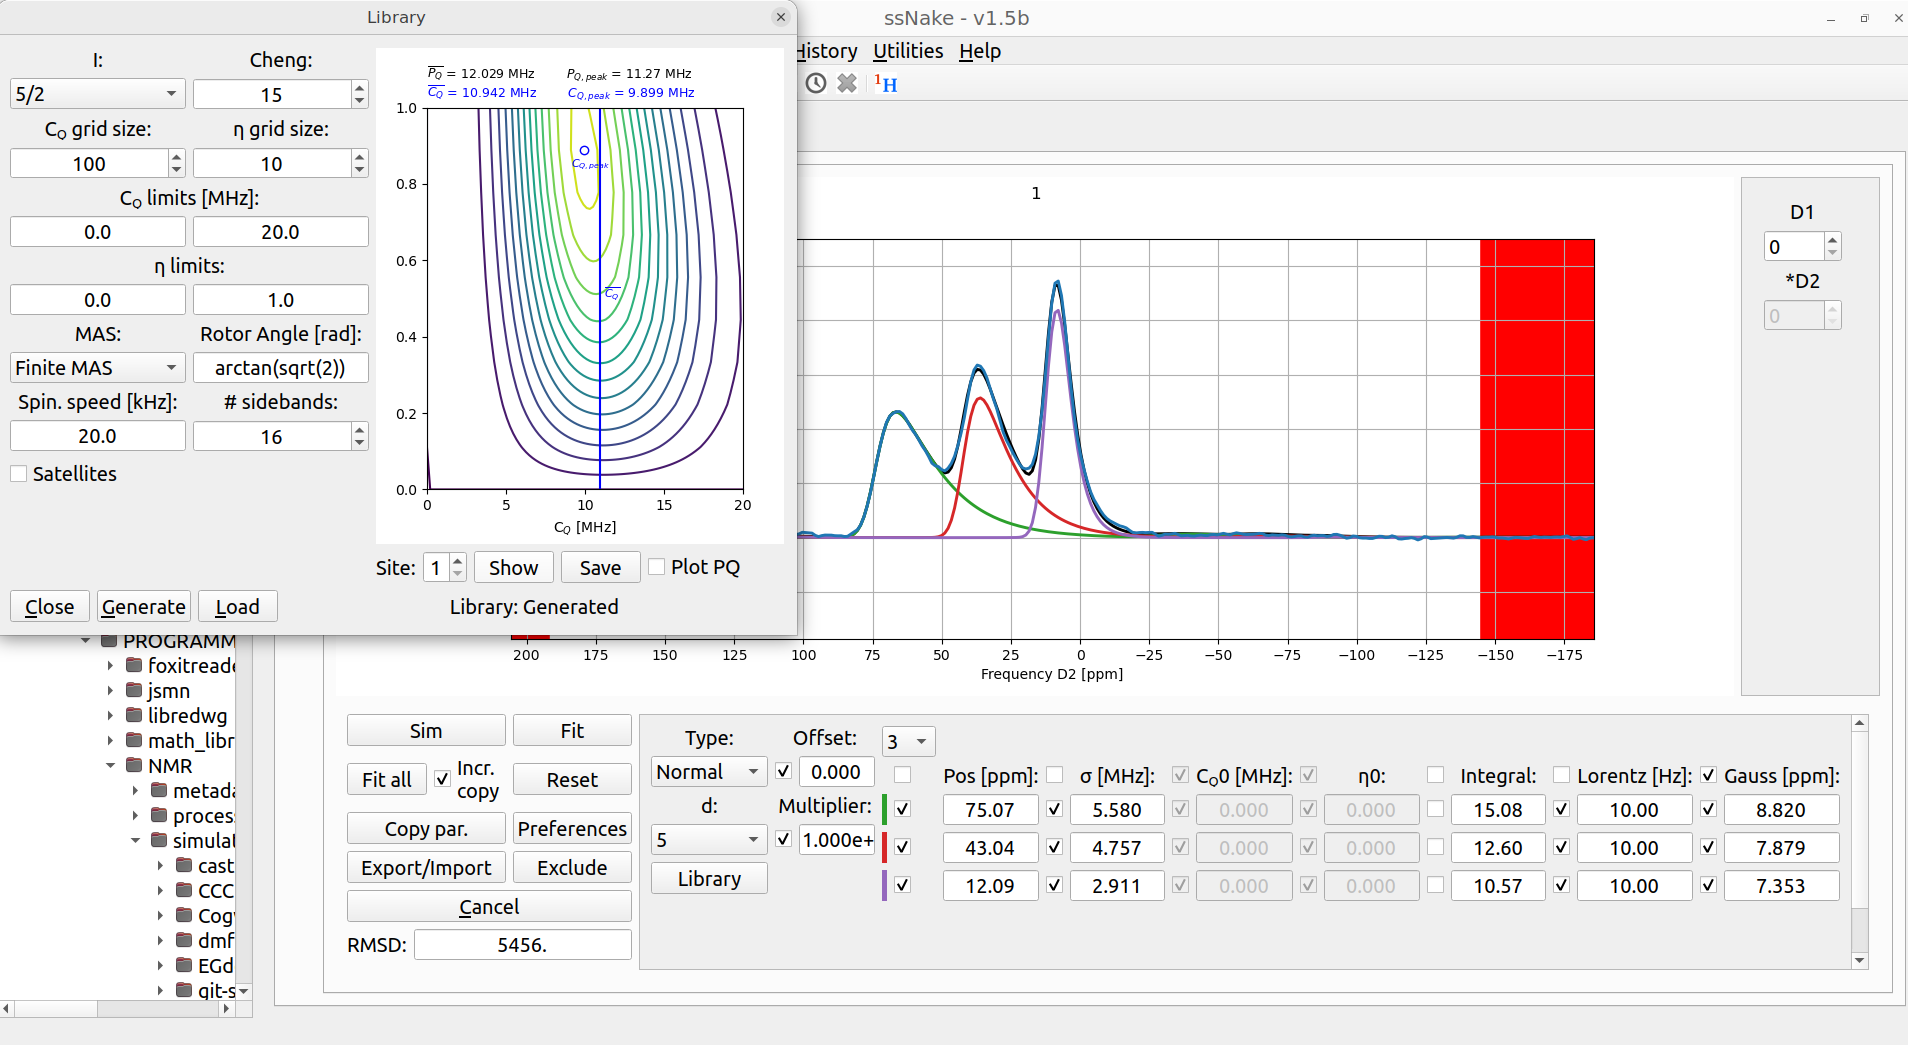
\includegraphics[width=0.8\linewidth]{Figs/FinalFit_1D.png}
%\end{center}
%%%
\end{document}
